\section{Text Mining Pipeline}
\label{sec:pipeline}
This section describes how the raw data is preprocessed in order to train a classifier that performs NER and NEL on German newspaper articles.
~\\
Preprocesing on Wikipedia dump\\
Explanation of jobs and their runtimes\\
Tools: Stanford CoreNLP (Tokenizer), Apache Lucene (Stemmer)\\
Data structures: Trie (for alias recognition)\\

\subsection{Raw data}
The system uses Wikipedia and Wikidata as data sources to train the classifier that performs NEL. The following will describe both of them.

\subsubsection{Wikipedia}
As project aims on analyzing German newspaper articles, the German Wikipedia provides appropriate training data. It currently consists of 3.6 million articles [source]. The articles have 3 main components: - Natural language text makes up most of the data. - Links to other Wikipedia pages. - Structured content, such as infoboxes.\\
The system will train the classifier based on the text and the links. It discards the structured content, as most of it is part of DBpedia [source], which is already included in the company graph [source reference to other BA].\\
For faster processing, the system accesses this data via a dump of the Wikipedia [source link] that consists of XML and Wikimarkup. The whole dump has a size of 15.9 GiB.

\subsubsection{Wikidata}
The German Wikidata [source link] describes the same entities as the German Wikipedia. But in contrast to Wikipedia, it does not provide a textual description but an ontology for them. This includes the class of an entity, which can be a business or an organization [todo concrete identifier]. This information is used to train the classifier only with relevant data.\\
As Wikipedia, the system also accesses the German Wikidata via a dump that is stored as JSON. It has a size of 90.2 GiB.

\subsection{Overview}
The preprocessing of the raw data consists of multiple steps as depicted in Fig.~\ref{fig:job_dependencies}. The system
- filters the data sources for their relevant content and stores this into tables of an Apache Cassandra database. (Parsing)
- refines the links within the Wikipedia and counts the references between each alias and entity. (Link analysis)
- searches for aliases of organizations in the Wikipedia text. (Alias analysis) 
- analyzes the frequencies of words in the Wikipedia text. (Word analysis)
%- generates features to train the classifier. (Feature generation)
%- trains the classifier. (Classifier training)
%- performs NEL on newspaper articles. (NEL)

\begin{figure}[ht]
	\centering
  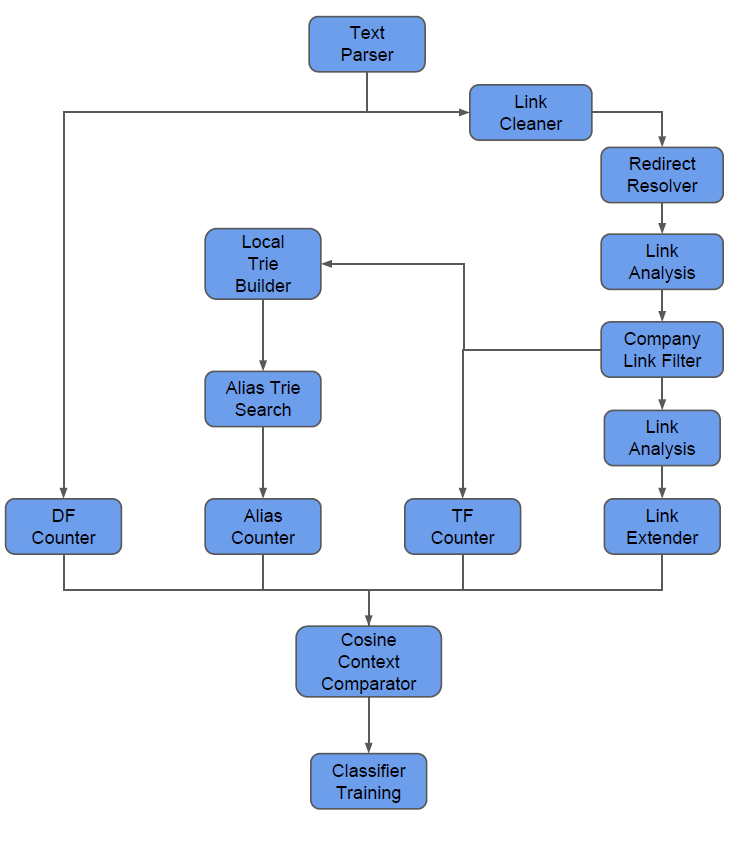
\includegraphics[width=0.7\textwidth]{Graphics/job_dependencies.png}
	\caption{Dependencies between the jobs of the text mining pipeline}
	\label{fig:job_dependencies}
\end{figure}


\subsection{Data preprocessing}
This subsection describes how the presented steps work in detail.

\subsubsection{Parsing}
For each article in Wikipedia, the parsing step converts the Wikimarkup to HTML by means of [source tool]. It then extracts the raw text and saves it into an entry in a Cassandra table. It also saves the contained links to other Wikipedia entities separately.

\subsubsection{Link analysis}
\subsubsection{Alias analysis}
\subsubsection{Word analysis}

\paragraph{Text parser}
\paragraph{Link cleaner}
\paragraph{Redirect resolver}
\paragraph{Link analysis}
\paragraph{Company link filter}
\paragraph{Link extender}
\paragraph{Trie builder}
\paragraph{Alias trie search}
\paragraph{Alias counter}
\paragraph{Document frequency counter}
\paragraph{Term frequency counter}
\paragraph{Cosine context comparator}

\subsection{Classifier training}
details following in the next section